\documentclass[12pt]{article}

\usepackage{sbc-template}
\usepackage{graphicx,url,amsmath,amssymb,booktabs,float}
\usepackage[brazilian]{babel}
\usepackage[utf8]{inputenc}
\usepackage[T1]{fontenc}

\sloppy

\title{Explorando o Paralelismo em Random Forests: Desempenho,\\
Fidelidade Preditiva e Eficiência Energética com OpenMP}

\author{Gabriel L. Bonavina\inst{1}, Estevan T. Santos\inst{1},\\
Marcelo F. Ohno\inst{1}, Vinicius M. Goulart\inst{1}}

% Mesmo efeito do \email do template, com os e-mails em 2 colunas.
\address{Universidade Federal de São Paulo (Unifesp)\\\mbox{}\\[-6pt]
  \footnotesize\ttfamily
  \begin{tabular}{@{}l@{\hspace{2.5em}}l@{}}
    gabriel.bonavina@unifesp.br & estevan.santos@unifesp.br \\
    marcelo.ohno@unifesp.br     & vmgoulart07@unifesp.br
  \end{tabular}}

\begin{document}

\maketitle

\begin{abstract}
Random Forest aggregates decision trees trained on bootstrap samples, evaluating
random feature subsets at each split and determining predictions by majority vote.
Sorting candidate splits at each internal node dominates training runtime, while
the trees themselves are independent. This paper measures the strong scaling of
one OpenMP implementation on four benchmarks (150 to 581{,}012 samples), from 1
to 32 threads, on a 6-core, 12-thread Intel Core i7-9750H. Training speedup reaches
7.32$\times$ on Covertype and 7.19$\times$ on Letter Recognition, and the CPU
package energy-delay product falls by up to 20.8$\times$. On the small sets the
curve peaks earlier and declines once the thread count exceeds the available work.
Test accuracy stays within 0.07 percentage points of the single-thread result.
\end{abstract}

\begin{resumo}
O algoritmo Random Forest combina árvores de decisão induzidas sobre amostras
bootstrap, avaliando subconjuntos aleatórios de atributos em cada partição e
definindo a predição por voto majoritário. A ordenação dos cortes candidatos em
cada nó interno domina o treinamento, enquanto as árvores crescem de forma
independente. Este trabalho mede o escalonamento forte de uma implementação
OpenMP em quatro bases (150 a 581 mil instâncias), de 1 a 32 threads, em um
Intel Core i7-9750H de 6 núcleos e 12 threads. O treino acelera até 7{,}32$\times$ no
Covertype e 7{,}19$\times$ no Letter Recognition, e o produto energia-atraso do
pacote da CPU cai até 20{,}8$\times$. Nas bases pequenas a curva atinge o máximo
antes e recua quando o número de threads excede o trabalho disponível. A
acurácia de teste permanece a até 0{,}07 ponto percentual do resultado com uma
thread.
\end{resumo}

\section{Introdução}

A classificação supervisionada mapeia instâncias com atributos numéricos a classes
discretas, com ampla aplicação em diagnóstico médico, visão computacional e
sensoriamento remoto. Entre os métodos baseados em comitês (\textit{ensembles}), o
Random Forest~\cite{breiman:2001,breiman:1984} destaca-se pela alta acurácia preditiva
e robustez ao sobreajuste por meio da agregação de múltiplas árvores de decisão.

A indução de florestas sobre bases volumosas impõe elevado custo computacional. O
algoritmo exibe paralelismo de dois grãos: as árvores crescem de forma independente,
mas a construção de cada nó exige ordenações sucessivas. Este artigo avalia o
escalonamento forte de uma implementação OpenMP~\cite{openmp:2018} quanto a tempo
de execução, acurácia e Produto Energia-Atraso (EDP)~\cite{gonzalez:1996}, com a
energia do pacote da CPU lida pelo Intel RAPL~\cite{david:2010}, em bases de 150 a
581{.}012 instâncias e com 1, 2, 4, 8, 16 e 32 threads.

\section{Random Forest}
\label{sec:rf}

\subsection{Árvore de decisão}

O conjunto de treino compreende amostras $(x_i, y_i)$, onde cada vetor
$x_i \in \mathbb{R}^d$ representa uma instância de $d$ atributos contínuos e
$y_i \in \{1, \dots, K\}$ denota sua classe entre $K$ categorias. Uma árvore de
classificação e regressão (CART)~\cite{breiman:1984} particiona o espaço de
atributos recursivamente por meio de testes univariados da forma $x_f \le \theta$,
com $f \in \{1, \dots, d\}$ e $\theta \in \mathbb{R}$. Instâncias que satisfazem a
desigualdade seguem para o filho esquerdo, e as demais para o direito. A
Figura~\ref{fig:arvore} ilustra uma árvore induzida no Iris, em que o nó raiz
avalia o atributo 2 com limiar 2{,}35, e as folhas definem a classe predita.

\begin{figure}[!ht]
\centering
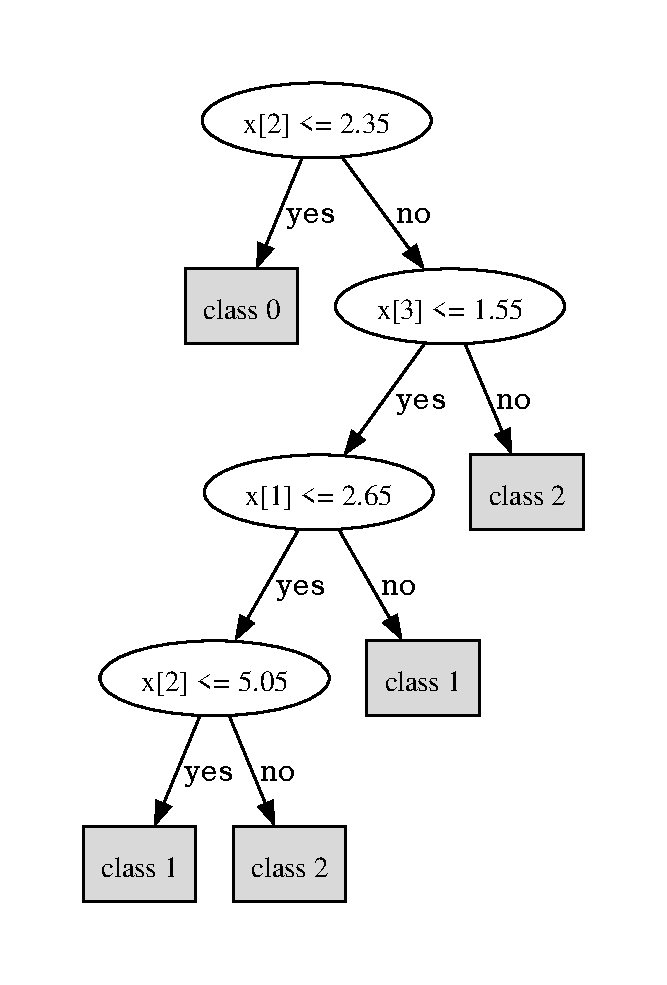
\includegraphics[width=0.35\textwidth]{figuras/arvore_iris.pdf}
\caption{Árvore ilustrativa induzida no Iris. Atributos numerados a partir de zero;
cada folha devolve a classe majoritária entre os exemplos que a alcançam.}
\label{fig:arvore}
\end{figure}

Em cada nó interno com subconjunto de amostras $S$, o corte ideal maximiza a
homogeneidade das partições geradas, mensurada pela impureza de Gini. Sendo $p_k$ a
fração empírica de instâncias da classe $k$ em $S$, $I_G(S) = 1 - \sum_{k=1}^{K} p_k^2$.
Um nó puro exibe $I_G = 0$, enquanto a divisão equilibrada entre duas classes resulta
em $I_G = 0{,}5$. Ao avaliar um candidato que divide $S$ em $S_L$ e $S_R$, calcula-se a
impureza média ponderada
$I_G(S, f, \theta) = \frac{|S_L|}{|S|} I_G(S_L) + \frac{|S_R|}{|S|} I_G(S_R)$, elegendo-se
o corte de menor valor. Na implementação, ordenam-se os valores do atributo $f$ nas linhas
de $S$ e os limiares posicionam-se no ponto médio entre valores adjacentes distintos. A
recursão cessa se o nó for puro, se $|S| < n_{\min}$, ou na profundidade máxima $D$,
atribuindo-se à folha a classe majoritária. Árvores profundas têm alta variância.

\subsection{Da árvore à floresta}

O Random Forest atenua essa variância combinando $T$ árvores de decisão
descorrelacionadas~\cite{breiman:2001} por meio de dois mecanismos estocásticos:
(i)~\textit{bootstrap aggregating (bagging)}~\cite{breiman:1996}, onde cada árvore é
induzida sobre $N$ amostras sorteadas com reposição (cerca de 63{,}2\% das instâncias
originais); e (ii)~\textit{subespaço aleatório de atributos}, avaliando-se em cada nó
apenas $m \le d$ atributos sem reposição (tipicamente $m \approx \lfloor\sqrt{d}\rfloor$, passível de calibração), o que evita a
predominância de atributos fortes.

Na inferência, a amostra percorre cada árvore até uma folha, definindo a predição por
voto majoritário simples. Como as árvores não trocam dados durante o crescimento, o laço
de indução é embaraçosamente paralelo. A reprodutibilidade decorre do gerador xorshift32
com semente privativa $s_t = s + t \cdot \texttt{0x9E3779B9} + 1$ para a árvore $t$, com
$s = 42$ também na partição holdout estratificada (80\% treino e 20\% teste).

\section{Paralelização com OpenMP}
\label{sec:impl}

A implementação paraleliza dois laços e mantém sequencial o trabalho interno de cada
um. O tamanho do time é \texttt{OMP\_NUM\_THREADS}. Com \texttt{OMP\_DYNAMIC}
desligado, o runtime não reduz esse time durante a execução. A cláusula
\texttt{default(none)} obriga a classificar toda variável do laço como compartilhada
ou privativa, de modo que as escritas fiquem explícitas.

\subsection{Crescimento das árvores}

O treinamento percorre as $T$ árvores com
\texttt{\#pragma omp parallel for schedule(dynamic) default(none)} sobre o índice
$t$. Sem tamanho de bloco, o escalonamento dinâmico entrega uma árvore por vez: a
thread que termina pede o próximo índice. Cada árvore sorteia a própria amostra
bootstrap e a própria sequência de atributos, então o número de nós e o tempo de
cada ordenação variam. Um \texttt{schedule(static)} fixaria um bloco de índices no
início do laço, e a thread que recebesse várias árvores profundas seguraria a
barreira final enquanto as outras já tivessem terminado.

No caminho de sucesso, o que é compartilhado é somente leitura: o vetor de árvores,
a matriz de treino e os hiperparâmetros. O índice $t$ e a semente
$s_t = s + t \cdot \texttt{0x9E3779B9} + 1$ são privativos. A rotina que cresce a
árvore $t$ aloca, na thread que a executa, o vetor bootstrap, os contadores de classe
e a arena de nós daquela árvore. A ordenação de um atributo usa um vetor de pares
local. Nenhuma dessas estruturas é compartilhada, e o crescimento não entra em
região crítica. A única escrita compartilhada é a bandeira de falha de alocação,
atualizada com \texttt{\#pragma omp atomic write}. Na execução normal, a única
sincronização é a barreira implícita no fim do \texttt{parallel for}.

A semente depende do índice da árvore, não da thread que a constrói. Mudar o
escalonamento troca o núcleo que produz a árvore $t$, e preserva a sequência de
cortes associada a esse índice.

O laço interno, que percorre os $m$ atributos do nó e ordena os pares, permanece
sequencial. Um segundo \texttt{parallel for} aninhado repartiria um vetor curto
entre threads que o laço externo já distribuiu pelos núcleos. Por omissão, o runtime
também não forma um segundo time dentro de uma região que já está ativa. Várias
árvores crescem ao mesmo tempo lendo a mesma matriz de treino: as amostras bootstrap
se sobrepõem, e as ordenações disputam a cache de último nível e o controlador de
memória do chip. É esse compartilhamento de leitura, e não uma trava entre árvores,
que limita o speedup quando o número de threads se aproxima dos processadores
lógicos.

\subsection{Predição e acurácia}

Depois do treinamento os nós não mudam. A predição paraleliza as linhas, não as
árvores, com \texttt{\#pragma omp parallel for schedule(static) default(none)}.
Cada linha desce todas as árvores, num caminho de comprimento no máximo $D$, sobre
estruturas somente leitura. Como esse custo é regular, o escalonamento estático
divide as $n$ linhas em blocos contíguos de tamanho próximo de $n/p$, um bloco por
thread, sem roubo de trabalho. Linhas vizinhas ocupam posições vizinhas na matriz,
e o bloco contíguo reaproveita a cache.

A thread avalia uma linha por vez. O voto percorre as árvores em série e acumula a
classe da folha num vetor privativo; a classe majoritária é escrita só na posição
daquela linha. Paralelizar o voto de uma única linha pediria uma redução sobre as
$K$ classes e só se pagaria com uma amostra e muitas árvores. O laço externo já
distribui, nas bases grandes, dezenas ou centenas de milhares de linhas.

A acurácia percorre as predições com outro laço estático e
\texttt{reduction(+:ok)}. Cada thread soma os acertos do próprio bloco numa parcial
privativa, e o runtime adiciona as parciais ao fim do laço.

\subsection{Linha de base}

Todos os speedups usam este mesmo binário. Com uma thread o \texttt{parallel for}
continua no código, mas o time tem um único membro: a razão $T(1)/T(p)$ isola o
número de threads, e não a diferença entre dois programas. Quando $p$ passa de 12,
as threads excedentes dividem os 12 processadores lógicos por fatias de tempo do
sistema operacional.

\section{Metodologia experimental}
\label{sec:met}

Os conjuntos de dados são Iris~\cite{fisher:1936}, Wisconsin Diagnostic Breast Cancer
(WDBC)~\cite{street:1993}, Letter Recognition~\cite{frey:1991} e Forest
Covertype~\cite{blackard:1999}. Os hiperparâmetros de Iris, WDBC e Letter foram
calibrados por busca em grade, com a acurácia de teste média sobre várias sementes
de partição. Em Iris e WDBC, entre as configurações a até 0{,}0025 da melhor
acurácia média, escolheu-se a de mais árvores e, entre essas, a de menor tempo de
treino. No Letter adotou-se a configuração de maior acurácia média da grade. O
Covertype foi fixado em 50 árvores, profundidade 30 e $m = 18$. A
Tabela~\ref{tab:config} resume as dimensões, o holdout estratificado por classe
(80\% treino e 20\% teste) e a acurácia de teste medida com uma thread.

\begin{table}[H]
\centering
\caption{Partição holdout de 20\% e acurácia de teste com uma thread. O número
mínimo de amostras para partição ($n_{\min}$) é 5 para Iris e WDBC, e 2 para
Letter e Covertype.}
\label{tab:config}
\footnotesize
\setlength{\tabcolsep}{4pt}
\begin{tabular}{@{}lrrrrrrrr@{}}
\toprule
Conjunto & Treino & Teste & $d$ & $K$ & Árv. & Prof. & $m$ & Acurácia \\
\midrule
Iris     & 120      & 30       & 4  & 3  & 300 & 12 & 2  & 0{,}9333 \\
WDBC     & 455      & 114      & 30 & 2  & 300 & 6  & 3  & 0{,}9912 \\
Letter   & 16{.}000 & 4{.}000  & 16 & 26 & 300 & 30 & 4  & 0{,}9620 \\
Cover    & 464{.}809 & 116{.}203 & 54 & 7 & 50 & 30 & 18 & 0{,}9603 \\
\bottomrule
\end{tabular}
\end{table}

A varredura de escalonamento forte usa o mesmo binário OpenMP com
\texttt{OMP\_NUM\_THREADS} em $\{1, 2, 4, 8, 16, 32\}$ e \texttt{OMP\_DYNAMIC}
desligado, uma execução por configuração, semente 42. O speedup de uma etapa é a
razão entre o tempo com uma thread e o tempo com $p$ threads. O hardware é um
Intel Core i7-9750H sob Windows: 6 núcleos físicos com \textit{hyper-threading}
(12 threads lógicas), frequência de base 2{,}6\,GHz, turbo de até 4{,}5\,GHz,
12\,MB de cache L3 e TDP de 45\,W. Os pontos de 16 e 32 threads excedem as 12
threads lógicas.

A energia $E$ não é a do notebook inteiro. O Intel RAPL~\cite{david:2010} acumula
joules em domínios do chip. O domínio lido aqui é o \textit{package}, o
encapsulamento físico do processador: os seis núcleos, as caches e a lógica
compartilhada do chip, inclusive o controlador de memória
integrado e a interconexão entre os núcleos. O contador é amostrado em nanojoules
no início e no fim do processo; $E$ é a diferença, convertida para joules. A DRAM
permanece num domínio próprio do RAPL e não entra nessa diferença.

A potência média do pacote é $\bar{P} = E/\Delta t$, em watts. É a energia do
encapsulamento dividida pelo intervalo de parede da execução completa, medido do
lançamento ao término do processo, que inclui a leitura do arquivo, a partição, o
treino e a inferência. Não é a potência instantânea de um
núcleo, nem o consumo medido na tomada. Com uma thread o package já mantém ligados
a cache de último nível e o controlador de memória. Threads adicionais acordam
outros núcleos e elevam $\bar{P}$, mas não na proporção de $p$: a parte
compartilhada do chip não se replica por thread, e a segunda thread de um núcleo,
pelo \textit{hyper-threading}, divide unidades de execução que já estão ligadas.
O Produto Energia-Atraso é
$\mathrm{EDP} = E \cdot \Delta t$, e o speedup correspondente é
$S_{\mathrm{EDP}} = E_1 \Delta t_1 / E_p \Delta t_p$. Os tempos de treino e de
predição vêm dos cronômetros internos do programa. O tempo de predição cobre a
inferência sobre os conjuntos de treino e de teste, usada no cálculo das duas
acurácias. Como o contador RAPL
atualiza-se na escala de dezenas de milissegundos, execuções inferiores a cerca de
0{,}5\,s (Iris, e parte do WDBC) ficam no piso de sensibilidade do medidor; as
conclusões energéticas apoiam-se em Letter e Covertype.

\section{Resultados}
\label{sec:res}

A Figura~\ref{fig:speedup} mostra a curva de speedup do treinamento, e a
Tabela~\ref{tab:treino} lista os tempos e os fatores correspondentes. Em Letter e
Covertype a curva acompanha a reta linear até 4 threads (eficiência de 0{,}95 e
0{,}92), continua subindo até 16 threads e estabiliza em 32: 7{,}19$\times$ no
Letter (19{,}50\,s para 2{,}71\,s) e 7{,}32$\times$ no Covertype (510{,}8\,s para
69{,}7\,s). No WDBC o máximo é 6{,}15$\times$ em 16 threads (0{,}406\,s para
0{,}066\,s), com recuo para 4{,}67$\times$ em 32. No Iris, cujo treino com uma
thread dura 26\,ms, o máximo é 2{,}89$\times$ em 8 threads e o ponto de 32 threads
volta a 1{,}13$\times$.

\begin{table}[H]
\centering
\caption{Tempo de treinamento (s) e speedup sobre a execução com uma thread.}
\label{tab:treino}
\footnotesize
\setlength{\tabcolsep}{4.5pt}
\begin{tabular}{@{}llrrrrrr@{}}
\toprule
Conjunto & & 1 & 2 & 4 & 8 & 16 & 32 \\
\midrule
Iris   & $t$ & 0{,}026 & 0{,}013 & 0{,}023 & 0{,}009 & 0{,}011 & 0{,}023 \\
       & $S$ & 1{,}00  & 2{,}00  & 1{,}13  & 2{,}89  & 2{,}36  & 1{,}13  \\
WDBC   & $t$ & 0{,}406 & 0{,}256 & 0{,}169 & 0{,}085 & 0{,}066 & 0{,}087 \\
       & $S$ & 1{,}00  & 1{,}59  & 2{,}40  & 4{,}78  & 6{,}15  & 4{,}67  \\
Letter & $t$ & 19{,}50 & 9{,}89  & 5{,}12  & 3{,}27  & 2{,}84  & 2{,}71  \\
       & $S$ & 1{,}00  & 1{,}97  & 3{,}81  & 5{,}96  & 6{,}87  & 7{,}19  \\
Cover  & $t$ & 510{,}8 & 267{,}5 & 138{,}7 & 95{,}16 & 70{,}79 & 69{,}74 \\
       & $S$ & 1{,}00  & 1{,}91  & 3{,}68  & 5{,}37  & 7{,}22  & 7{,}32  \\
\bottomrule
\end{tabular}
\end{table}

O intervalo do processo inteiro, o mesmo $\Delta t$ usado em $\bar{P}$ e no EDP,
acelera menos que o treino porque inclui a leitura do arquivo e a partição
holdout, que são sequenciais (entre 23 e 26\,s no Covertype, com qualquer número
de threads). No Covertype ele passa de 557{,}0\,s para 94{,}9\,s (5{,}87$\times$ em
32 threads); no Letter, de 22{,}27\,s para 3{,}35\,s (6{,}64$\times$).

Na predição, Letter passa de 2{,}38\,s para 0{,}28\,s (8{,}43$\times$ em 32
threads) e Covertype de 19{,}91\,s para 1{,}70\,s (11{,}75$\times$). A
Tabela~\ref{tab:pred} detalha essa etapa. O ganho supera o do treino porque o
custo por amostra é uniforme e o escalonamento estático reparte linhas somente de
leitura. No Covertype o speedup de 2 threads (2{,}51$\times$) já fica acima do
linear; com uma execução por ponto, parte desse excedente pode vir de variação na
execução de referência, e não do paralelismo. No Iris e no WDBC a predição dura
entre 0 e 13\,ms, na resolução do cronômetro interno, e esses pontos não entram na
curva.

\begin{figure}[H]
\centering
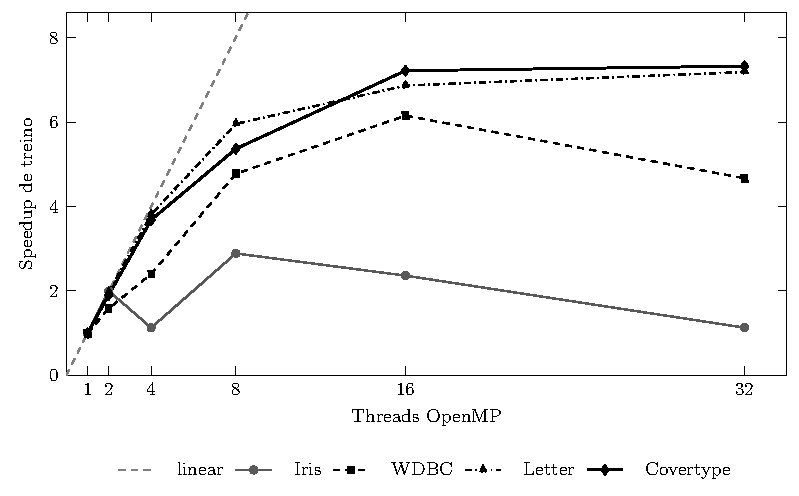
\includegraphics[width=\textwidth]{figuras/speedup.pdf}
\caption{Speedup de treinamento em relação à mesma implementação OpenMP com uma
thread. A reta tracejada é o speedup linear. Letter e Covertype sobem até cerca
de 7$\times$ e estabilizam entre 16 e 32 threads. Iris e WDBC, com treino abaixo
de meio segundo, atingem o máximo antes e recuam em 32 threads.}
\label{fig:speedup}
\end{figure}

\begin{table}[H]
\centering
\caption{Tempo de predição (s), sobre os conjuntos de treino e de teste, e speedup
sobre a execução com uma thread, nas bases em que o cronômetro resolve a etapa.}
\label{tab:pred}
\footnotesize
\setlength{\tabcolsep}{4.5pt}
\begin{tabular}{@{}llrrrrrr@{}}
\toprule
Conjunto & & 1 & 2 & 4 & 8 & 16 & 32 \\
\midrule
Letter & $t$ & 2{,}38 & 1{,}24 & 0{,}66 & 0{,}36 & 0{,}29 & 0{,}28 \\
       & $S$ & 1{,}00 & 1{,}91 & 3{,}59 & 6{,}57 & 8{,}20 & 8{,}43 \\
Cover  & $t$ & 19{,}91 & 7{,}94 & 4{,}30 & 2{,}53 & 1{,}84 & 1{,}70 \\
       & $S$ & 1{,}00 & 2{,}51 & 4{,}63 & 7{,}87 & 10{,}80 & 11{,}75 \\
\bottomrule
\end{tabular}
\end{table}

A Tabela~\ref{tab:energia} reúne a energia do pacote e o speedup de EDP, e a
Figura~\ref{fig:edp} compara os dois fatores. No
Letter, a energia cai de 53{,}1\,J para 24{,}5\,J em 32 threads e o EDP melhora
14{,}4$\times$. No Covertype, a energia cai de 2{.}085\,J para 588\,J e o EDP
melhora 20{,}8$\times$. A potência média do pacote, $\bar{P} = E/\Delta t$, sobe
menos do que o tempo cai: no Letter, de 2{,}38\,W com uma thread para 7{,}31\,W
com 32; no Covertype, de 3{,}74\,W para 6{,}20\,W. O encurtamento da execução,
somado a esse aumento moderado da energia por segundo do chip, reduz ao mesmo
tempo a energia total e o atraso. A acurácia de teste não
depende do número de threads de forma material. Iris e WDBC repetem 0{,}9333 e
0{,}9912 em todos os pontos. Letter permanece no intervalo 0{,}9613--0{,}9627 e
Covertype no intervalo 0{,}9599--0{,}9603, isto é, a até 0{,}07 ponto
percentual do valor com uma thread.

\begin{table}[H]
\centering
\caption{Energia do pacote da CPU (J) e speedup de EDP sobre a execução com uma
thread. Letter e Covertype estão acima do piso de resolução do RAPL. Iris (0{,}15
a 0{,}59\,J) e WDBC (1{,}4 a 4{,}0\,J) ficam no piso, com $S_{\mathrm{EDP}}$ não
monótono, e não são listados.}
\label{tab:energia}
\footnotesize
\setlength{\tabcolsep}{4.2pt}
\begin{tabular}{@{}llrrrrrr@{}}
\toprule
Conjunto & & 1 & 2 & 4 & 8 & 16 & 32 \\
\midrule
Letter & $E$ & 53{,}1 & 42{,}1 & 32{,}5 & 28{,}5 & 26{,}6 & 24{,}5 \\
       & $S_{\mathrm{EDP}}$ & 1{,}00 & 2{,}44 & 5{,}92 & 10{,}36 & 12{,}81 & 14{,}36 \\
Cover  & $E$ & 2{.}085 & 1{.}396 & 900 & 768 & 623 & 588 \\
       & $S_{\mathrm{EDP}}$ & 1{,}00 & 2{,}76 & 7{,}76 & 12{,}43 & 19{,}27 & 20{,}81 \\
\bottomrule
\end{tabular}
\end{table}

\begin{figure}[H]
\centering
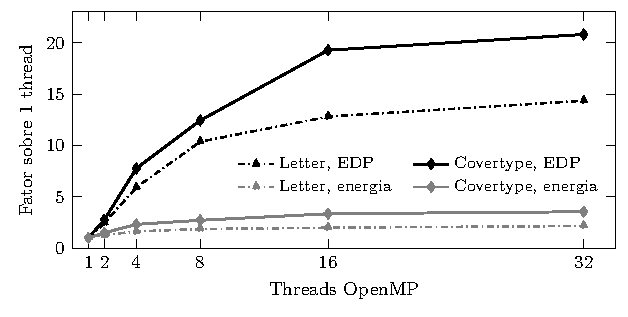
\includegraphics[width=0.72\textwidth]{figuras/edp.pdf}
\caption{Redução da energia do pacote ($E_1/E_p$, em cinza) e speedup de EDP (em
preto) sobre a execução com uma thread, em Letter e Covertype. O EDP cresce mais
que a energia porque multiplica a redução de energia pela redução de tempo.}
\label{fig:edp}
\end{figure}

\section{Discussão}
\label{sec:disc}

O treinamento escala enquanto há árvores independentes e núcleos capazes de
ordená-las ao mesmo tempo. Até 4 threads, Letter e Covertype ficam próximos da
reta linear (eficiência de 0{,}95 e 0{,}92): quatro threads ocupam quatro dos seis
núcleos físicos, cada uma com o núcleo inteiro. De 4 para 8 threads a eficiência
cai para 0{,}74 no Letter e 0{,}67 no Covertype. Oito threads já passam dos seis
núcleos, e pelo menos dois deles executam duas threads por \textit{hyper-threading},
dividindo unidades de execução e as caches L1 e L2. De 8 para 16 threads o ganho
continua, de 5{,}37$\times$ para 7{,}22$\times$ no Covertype, embora 16 já ultrapasse
as 12 threads lógicas; de 16 para 32 o treino das bases grandes praticamente para
(7{,}22$\times$ para 7{,}32$\times$ no Covertype). O teto fica acima dos seis núcleos
físicos e abaixo das doze threads lógicas: o \textit{hyper-threading} acrescenta
vazão sem dobrá-la, as ordenações disputam a banda de memória, e, acima de 12
threads, as threads excedentes compartilham os mesmos processadores lógicos. O
escalonamento dinâmico absorve a diferença de tamanho entre árvores, sem eliminar
esse teto.

Nas bases pequenas o mesmo mecanismo aparece mais cedo. O WDBC, com 455 amostras
de treino, ainda chega a 6{,}15$\times$ em 16 threads e perde terreno em 32, quando
o custo de acordar threads e de repartir 300 árvores curtas supera o trabalho de
cada uma. O Iris, com 120 amostras e 26\,ms de treino sequencial, oscila entre
1{,}13$\times$ e 2{,}89$\times$: a maior parte do tempo medido é overhead, não
ordenação. A predição, por outro lado, reparte dezenas ou centenas de milhares de
amostras de custo uniforme. Por isso o Covertype chega a 11{,}75$\times$ na
inferência com 32 threads, acima do speedup de treino, mesmo sobre 12 threads
lógicas: o laço é curto, regular e limitado sobretudo pela leitura das árvores.

O EDP acompanha essa assimetria entre tempo e potência do pacote. No Covertype,
$\bar{P}$ sobe de 3{,}74\,W para 6{,}20\,W (1{,}7 vezes): uma thread já paga a
cache e o controlador de memória, e as threads seguintes só acrescentam núcleos em
cima dessa base. O intervalo medido do processo encolhe o bastante para a energia
cair de 2{.}085\,J para 588\,J. O
produto dos dois efeitos é o speedup de EDP de 20{,}8$\times$, maior que o speedup
de tempo. O Letter repete o padrão em menor escala (14{,}4$\times$). Acrescentar
threads além de 16 melhora pouco o EDP dessas duas bases e não se justifica nas
bases cujo tempo já está no piso do sensor.

\section{Conclusão}
\label{sec:conc}

A varredura de 1 a 32 threads mostra que o Random Forest em OpenMP aproveita os
núcleos enquanto o treinamento é dominado por árvores independentes. Em Letter e
Covertype o treino acelera até 7{,}19$\times$ e 7{,}32$\times$, a predição até
8{,}43$\times$ e 11{,}75$\times$, e o EDP do pacote da CPU até 14{,}4$\times$ e
20{,}8$\times$, com a acurácia de teste estável. A curva é quase linear até 4
threads, ainda sobe até 16 e satura em 32, acima das 12 threads lógicas do
i7-9750H. Em Iris e WDBC o máximo ocorre antes e o excesso de threads aumenta o
tempo.

O arranjo prático, neste processador, é usar de 8 a 16 threads nas bases em que a
ordenação dos cortes domina o tempo, e poucas threads quando o treino dura frações
de segundo. Trabalhos futuros podem fixar uma thread por núcleo físico, para
separar o efeito do \textit{hyper-threading}, e repetir a varredura em
processadores com mais núcleos.

\bibliographystyle{sbc}
\bibliography{artigo}

\end{document}
